
\documentclass{beamer}

\usepackage{algpseudocode, color, colortbl}

\usepackage{hyperref}
\hypersetup{
    colorlinks=true,
    urlcolor=blue,
}

\usepackage{listings}

\usepackage{tikz}

\usetheme{Montpellier}
\usecolortheme{rose}

% page numbers, from
% https://tex.stackexchange.com/questions/137022/how-to-insert-page-number-in-beamer-navigation-symbols
\expandafter\def\expandafter\insertshorttitle\expandafter{%
  \insertshorttitle\hfill%
  \insertframenumber\,/\,\inserttotalframenumber}

\definecolor{Gray}{gray}{0.8}
\newcolumntype{g}{>{\columncolor{Gray}}c}

\newcommand{\stanza}{ \\~\ }

\title{07. Maximum Flow Formulations and Bipartite Matching}
\subtitle{CPSC 535}
\author{Kevin A. Wortman}
\institute{ \includegraphics[height=2cm]{csuf-logo-cmyk} }
\date{
\includegraphics[height=14pt]{by} \\

{\tiny
This work is licensed under a
\href{http://creativecommons.org/licenses/by/4.0/}{Creative Commons Attribution 4.0 International License}.
}}

\begin{document}

\begin{frame}
  \titlepage
\end{frame}

\begin{frame} \frametitle{Big Idea: Problem Reduction}
\emph{problem $A$ reduces to problem $B$} $=$ can use an algorithm for $B$ to do all the hard
work of solving problem $A$ \\
$= A$ is easier than $B$ (or tied) \stanza

Sometimes $A, B$ are closely related \\
e.g. $A = $ sorting bounded integers, $B = $ general sorting \stanza

More interesting: problems seem completely unrelated (e.g. SAT, CLIQUE;
max-flow, bipartite matching)
\end{frame}

\begin{frame} \frametitle{Reduction Algorithm Pseudocode}
  \emph{problem $A$ reduces to problem $B$} $=$ can use an algorithm for $B$ to do all the hard
  work of solving problem $A$ \stanza

  {\footnotesize
  \begin{algorithmic}[1]
    \Function{SOLVE-A}{input-for-A}
    \State input-for-B = pre-process input-for-A
    \State solution-for-B = solve-B(input-for-B)
    \State solution-for-A = post-process solution-for-B
    \State \Return{ solution-for-A }
    \EndFunction
  \end{algorithmic}
  }
\vspace{.5cm}
In spirit
\begin{itemize}
  \item the \textbf{solve-B} part is complex and the bottleneck
  \item the \textbf{overhead} (pre-process and post-process parts) is simple and fast
\end{itemize}
\end{frame}

\begin{frame} \frametitle{Reducing to Max-Flow}
  \textbf{maximum flow problem} \\
  \emph{input:} a flow network $G$ \\
  \emph{output:} a flow $f$ of maximum value $|f|$ \stanza

  {\footnotesize
  \begin{algorithmic}[1]
    \Function{SOLVE-A}{input-for-A}
    \State $G' = $ flow network based on input-for-A
    \State $f = $ SOLVE-MAX-FLOW($G'$)
    \State solution-for-A = post-process $f$
    \State \Return{ solution-for-A }
    \EndFunction
  \end{algorithmic}
  }
(use $G'$ because sometimes input-for-A is already a graph $G$) \stanza

The fastest max-flow alg. in CLRS takes $O(|V|^3)$ time; overhead usually takes
linear time; so SOLVE-MAX-FLOW is usually the bottleneck; $O(n^3)$ time
\end{frame}

\begin{frame} \frametitle{Formulation in General}
  To formulate $A$ as a $B$ instance, need to explain
  \begin{itemize}
  \item \emph{Input mapping:} how to map input-for-A to input-for-B
  \item \emph{Output mapping:} how to map solution-for-B to solution-for-A
  \item \emph{Correctness:} how
    \begin{itemize}
    \item all the ``rules'' of A are enforced...
    \item ......by the B problem itself, and/or our input mapping
    \end{itemize}
  \item ``rules:'' constraints on the output
  \item \emph{Overhead:} analyze whether the input/output mapping becomes the bottleneck
  \end{itemize}

  \vspace{.5cm}
  \textbf{This is a valuable problem-solving skill!}
\end{frame}

\begin{frame} \frametitle{Max-Flow Formulation}

\emph{Max-Flow Formulation:} details of how an algorithm for problem A
\begin{itemize}
  \item maps an input into a flow network $G'$
  \item recovers a solution from the flow $f$
\end{itemize}
\vspace{.5cm}
Also: analyze these steps to determine whether
\begin{itemize}
  \item overhead is $O(|V|^3)$ $\implies$ SOLVE-MAX-FLOW
    is the bottleneck in SOLVE-A (usually yes)
  \item or, overhead is $\Omega(|V|^3)$ and is the bottleneck
\end{itemize}
\vspace{.5cm}
Usually we only discuss these parts, and don't write out the SOLVE-A pseudocode
explicitly.
\end{frame}

\begin{frame} \frametitle{Max-Flow Formulation}
``Rules'' of problem $A$ must be implemented by the ``rules'' built
  into the max-flow problem and/or the edges and weights we introduce
\begin{itemize}
  \item directed graph $G=(V, E),$ source $s \in V,$ sink $t \in V$
  \item none of: self-loop, antiparallel edge, unreachable vertex
  \item non-negative capacity on every edge
  \item flow is function $f(u, v)$ over vertices $u, v$
  \item \textbf{nonexistent edges}: if $(u, v) \notin E$ then $f(u, v) = 0$
  \item \textbf{capacity constraint}: $0 \leq f(u, v) \leq c(u, v)$
  \item \textbf{flow conservation}: (flow-in) $=$ (flow-out), except for source and
    sink; formally, $\forall u \in V - \{s, t\},$
    \[ \sum_{v \in V} f(v, u) = \sum_{v \in V} f(u, v) \]
  \item \emph{value} $|f|$ = net flow into sink
  \end{itemize}
\end{frame}

\begin{frame} \frametitle{A Straightforward Formulation: Evacuation}
Suppose we are working with safety authorities to determine how quickly CSUF
could be evacuated in a natural disaster such as a wildfire. \stanza

\emph{evacuation rate problem} \\
\textbf{input:} directed graph $G$ representing a road map of Fullerton, each edge
weighted with the number of autos/hour that may travel on that road \\
\textbf{output:} the maximum number of autos/hour that could travel from CSUF to
a 57 or 91 freeway onramp \stanza

(Straightforward because this is clearly about flow in a directed graph.)
\end{frame}

\begin{frame} \frametitle{A Straightforward Formulation: Evacuation}
For a clear formulation, need to specify
\begin{itemize}
  \item how to convert road map into flow network $G';$ needs
  \begin{itemize}
    \item to be a directed graph
    \item source $s$ and sink $t$
    \item non-negative capacity on each edge
    \item no self-loops, antiparallel edges, or disconnected vertices
  \end{itemize}
  \item how to decode flow $f$ into a solution for our problem (\# autos/hour evacuated)
  \item overhead time efficiency
\end{itemize}
\end{frame}

\begin{frame} \frametitle{A Straightforward Formulation: Evacuation}
\begin{itemize}
  \item suppose for sake of discussion, road map $G$ has none of the taboo components (self-loops etc.)
  \item start with $G'=G$
  \item define source $s$ in $G'$ as the Gymnasium-Campus intersection on campus
  \item create new sink $t$ in $G'$ that represents ``on either freeway;''
    create edges from highway onramps to $t,$ each with capacity $\infty$
  \item after finding max-flow in $G',$ examine flow function $f$ to compute
    evacuation rate as
    \[ \sum_{\text{onramp vertex }o} f(o, t) \]
  \item overhead is $O(|V|+|E|),$ not bottleneck
\end{itemize}
\end{frame}

\begin{frame} \frametitle{Robust Max-Flow}
Goal: eliminate some of the pesky constraints of the classical max-flow problem
\stanza

\textbf{robust maximum flow problem} \\
\emph{input:} a flow network $G=(V,E),$ which may contain unreachable vertices,
antiparallel edges, a set $S \subseteq V$ of sources, and a set $T \subseteq V$
  of sinks\\
\emph{output:} a flow $f$ of maximum value $|f|$ \stanza
\vspace{.5cm}
\begin{itemize}
  \item unreachable vertices are allowed
  \item antiparallel edges are allowed
  \item \textbf{set} of sources/sinks instead of just one vertex each
\end{itemize}
\end{frame}

\begin{frame} \frametitle{Reformulating to Eliminate Unreachable Vertices}
given flow network $G$ that may contain unreachable vertices,
\begin{itemize}
  \item use BFS (or DFS) to mark every vertex that is reachable from $s$
  \item use BFS again, following edges backwards, to mark every vertex that is reachable from $t$
  \item if a vertex was not marked both times, it is redundant
  \item $G' = $ induced subgraph of $G$ with all redundant vertices removed
  \item compute flow $f'$ in $G'$
  \item to convert $f'$ to flow $f$ in $G$, set flow along all redundant edges to 0
  \item overhead is 2 $\times$ BFS $= O(|V|+|E|),$ not bottleneck
\end{itemize}
\end{frame}

\begin{frame} \frametitle{Reformulating to Eliminate Unreachable Vertices}
\begin{center}
\begin{tabular}{cccc}
$G$ & $G'$ & $f'$ & $f$ \\

% G
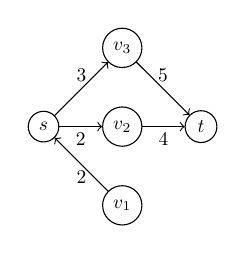
\begin{tikzpicture}[every node/.style={scale=.7}]
  \node [draw, circle] (s) at (0, 1) {$s$};
  \node [draw, circle] (v1) at (1, 0) {$v_1$};
  \node [draw, circle] (v2) at (1, 1) {$v_2$};
  \node [draw, circle] (v3) at (1, 2) {$v_3$};
  \node [draw, circle] (t) at (2, 1) {$t$};
  \draw [->] (s) -- node [below] {2} (v2);
  \draw [->] (s) -- node [above] {3} (v3);
  \draw [->] (v2) -- node [below] {4} (t);
  \draw [->] (v3) -- node [above] {5} (t);
  \draw [->] (v1) -- node [below] {2} (s);
\end{tikzpicture}

% G'
&
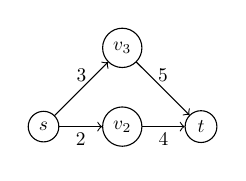
\begin{tikzpicture}[every node/.style={scale=.7}]
  \node [draw, circle] (s) at (0, 1) {$s$};
  \node [draw, circle] (v2) at (1, 1) {$v_2$};
  \node [draw, circle] (v3) at (1, 2) {$v_3$};
  \node [draw, circle] (t) at (2, 1) {$t$};
  \draw [->] (s) -- node [below] {2} (v2);
  \draw [->] (s) -- node [above] {3} (v3);
  \draw [->] (v2) -- node [below] {4} (t);
  \draw [->] (v3) -- node [above] {5} (t);
\end{tikzpicture}

% f'
&
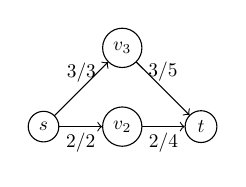
\begin{tikzpicture}[every node/.style={scale=.7}]
  \node [draw, circle] (s) at (0, 1) {$s$};
  \node [draw, circle] (v2) at (1, 1) {$v_2$};
  \node [draw, circle] (v3) at (1, 2) {$v_3$};
  \node [draw, circle] (t) at (2, 1) {$t$};
  \draw [->] (s) -- node [below] {2/2} (v2);
  \draw [->] (s) -- node [above] {3/3} (v3);
  \draw [->] (v2) -- node [below] {2/4} (t);
  \draw [->] (v3) -- node [above] {3/5} (t);
\end{tikzpicture}

% f
&
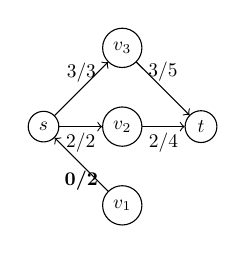
\begin{tikzpicture}[every node/.style={scale=.7}]
  \node [draw, circle] (s) at (0, 1) {$s$};
  \node [draw, circle] (v1) at (1, 0) {$v_1$};
  \node [draw, circle] (v2) at (1, 1) {$v_2$};
  \node [draw, circle] (v3) at (1, 2) {$v_3$};
  \node [draw, circle] (t) at (2, 1) {$t$};
  \draw [->] (s) -- node [below] {2/2} (v2);
  \draw [->] (s) -- node [above] {3/3} (v3);
  \draw [->] (v2) -- node [below] {2/4} (t);
  \draw [->] (v3) -- node [above] {3/5} (t);
  \draw [->] (v1) -- node [below] {\textbf{0/2}} (s);
\end{tikzpicture}

\end{tabular}
\end{center}
\end{frame}

\begin{frame} \frametitle{Reformulating to Eliminate Antiparallel Edges}
given a flow network $G$ that may contain antiparallel edges,
\begin{itemize}
  \item initially $G' = G$
  \item identify all antiparallel edges
  \item when $\exists$ antiparallel edges between vertices $v_1, v_2,$
  \begin{itemize}
    \item create new vertex $v'$ in $G'$ between $v_1, v_2$
    \item replace edge $(v_1, v_2)$ with edges $(v_1, v')$ and $(v', v_2)$
    \item set $c(v_1, v')=c(v', v_2)=c(v_1, v_2)$
  \end{itemize}
  \item observe that flow between $v_1, v_2$ is identical but antiparallel
    edge is eliminated
  \item to convert flow $f'$ in $G'$ to equiv. flow in $G:$ for each $v'$
    introduced above, set $f(v_1, v_2) = f'(v_1, v')$
  \item overhead is $O(|E|),$ $|E'| < 2|E| \in \Theta(|E|),$ not bottleneck
\end{itemize}
\end{frame}

\begin{frame} \frametitle{Reformulating to Eliminate Antiparallel Edges}
  \begin{center}
  \begin{tabular}{cccc}
  $G$ & $G'$ & $f'$ & $f$ \\

  % G
  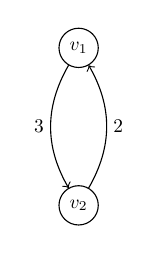
\begin{tikzpicture}[every node/.style={scale=.7}]
    \node [draw, circle] (v1) at (0, 2) {$v_1$};
    \node [draw, circle] (v2) at (0, 0) {$v_2$};
    \draw [->] (v1) to[bend right] node [left] {3} (v2);
    \draw [->] (v2) to[bend right] node [right] {2} (v1);
  \end{tikzpicture}

  % G'
  &
  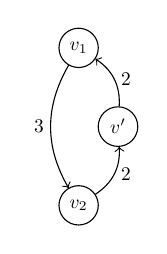
\begin{tikzpicture}[every node/.style={scale=.7}]
    \node [draw, circle] (v1) at (0, 2) {$v_1$};
    \node [draw, circle] (v2) at (0, 0) {$v_2$};
    \node [draw, circle] (v') at (.5, 1) {$v'$};
    \draw [->] (v1) to[bend right] node [left] {3} (v2);
    \draw [->] (v2) to[bend right] node [right] {2} (v');
    \draw [->] (v') to[bend right] node [right] {2} (v1);
  \end{tikzpicture}

  % f'
  &
  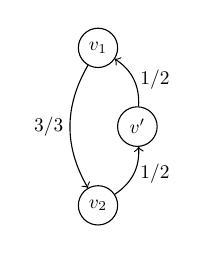
\begin{tikzpicture}[every node/.style={scale=.7}]
    \node [draw, circle] (v1) at (0, 2) {$v_1$};
    \node [draw, circle] (v2) at (0, 0) {$v_2$};
    \node [draw, circle] (v') at (.5, 1) {$v'$};
    \draw [->] (v1) to[bend right] node [left] {3/3} (v2);
    \draw [->] (v2) to[bend right] node [right] {1/2} (v');
    \draw [->] (v') to[bend right] node [right] {1/2} (v1);
  \end{tikzpicture}

  % f
  &
  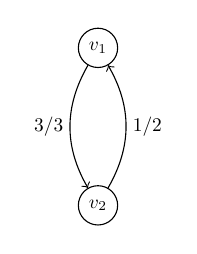
\begin{tikzpicture}[every node/.style={scale=.7}]
    \node [draw, circle] (v1) at (0, 2) {$v_1$};
    \node [draw, circle] (v2) at (0, 0) {$v_2$};
    \draw [->] (v1) to[bend right] node [left] {3/3} (v2);
    \draw [->] (v2) to[bend right] node [right] {1/2} (v1);
  \end{tikzpicture}

  \end{tabular}
  \end{center}
\end{frame}

\begin{frame} \frametitle{Reformulating to Accommodate Multiple Sinks or Sources}
  \begin{itemize}
    \item initially $G'=G$
    \item create in $G'$ a \emph{super-source} vertex $s$ and \emph{super-sink} $t$
    \item for each source $s_i \in G,$ create an edge $(s, s_i)$ in $G'$ with capacity
      $c(s, s_i) = \infty$
    \item for each sink $t_i \in G,$ create an edge $(t_i, t)$ in $G'$ with capacity
      $c(t_i, t) = \infty$
    \item to convert flow $f'$ in $G'$ to equiv. flow $f$ in $G:$ delete flow info.
      along any of the new edges
    \item overhead is $O(|V|), |V'|=|V|+2 \in \Theta(|V|), |E'| \leq |V|+|E|,$ not bottleneck
  \end{itemize}
\end{frame}

\begin{frame} \frametitle{Reformulating to Accommodate Multiple Sinks or Sources}
  \begin{center}
  \begin{tabular}{cccc}
  $G$ & $G'$ & $f'$ & $f$ \\

  % G
  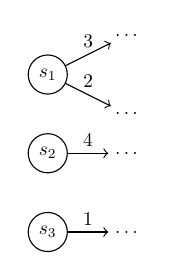
\begin{tikzpicture}[every node/.style={scale=.7}]
    \node [draw, circle] (s1) at (0, 2) {$s_1$};
    \node [draw, circle] (s2) at (0, 1) {$s_2$};
    \node [draw, circle] (s3) at (0, 0) {$s_3$};
    \node (v1) at (1, 2.5) {$\ldots$};
    \node (v2) at (1, 1.5) {$\ldots$};
    \node (v3) at (1, 1) {$\ldots$};
    \node (v4) at (1, 0) {$\ldots$};
    \draw [->] (s1) to node [above] {3} (v1);
    \draw [->] (s1) to node [above] {2} (v2);
    \draw [->] (s2) to node [above] {4} (v3);
    \draw [->] (s3) to node [above] {1} (v4);
  \end{tikzpicture}

  % G'
  &
  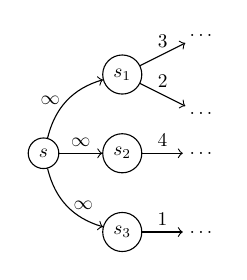
\begin{tikzpicture}[every node/.style={scale=.7}]
    \node [draw, circle] (s1) at (0, 2) {$s_1$};
    \node [draw, circle] (s2) at (0, 1) {$s_2$};
    \node [draw, circle] (s3) at (0, 0) {$s_3$};
    \node (v1) at (1, 2.5) {$\ldots$};
    \node (v2) at (1, 1.5) {$\ldots$};
    \node (v3) at (1, 1) {$\ldots$};
    \node (v4) at (1, 0) {$\ldots$};
    \draw [->] (s1) to node [above] {3} (v1);
    \draw [->] (s1) to node [above] {2} (v2);
    \draw [->] (s2) to node [above] {4} (v3);
    \draw [->] (s3) to node [above] {1} (v4);

    \node [draw, circle] (s) at (-1, 1) {$s$};
    \draw [->] (s) to[bend left] node [left] {$\infty$} (s1);
    \draw [->] (s) to node [above] {$\infty$} (s2);
    \draw [->] (s) to[bend right] node [right] {$\infty$} (s3);
  \end{tikzpicture}

  % f'
  &
  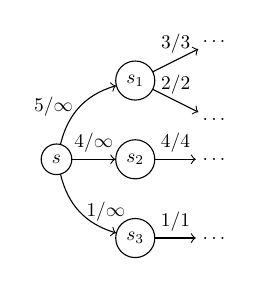
\begin{tikzpicture}[every node/.style={scale=.7}]
    \node [draw, circle] (s1) at (0, 2) {$s_1$};
    \node [draw, circle] (s2) at (0, 1) {$s_2$};
    \node [draw, circle] (s3) at (0, 0) {$s_3$};
    \node (v1) at (1, 2.5) {$\ldots$};
    \node (v2) at (1, 1.5) {$\ldots$};
    \node (v3) at (1, 1) {$\ldots$};
    \node (v4) at (1, 0) {$\ldots$};
    \draw [->] (s1) to node [above] {3/3} (v1);
    \draw [->] (s1) to node [above] {2/2} (v2);
    \draw [->] (s2) to node [above] {4/4} (v3);
    \draw [->] (s3) to node [above] {1/1} (v4);

    \node [draw, circle] (s) at (-1, 1) {$s$};
    \draw [->] (s) to[bend left] node [left] {5/$\infty$} (s1);
    \draw [->] (s) to node [above] {4/$\infty$} (s2);
    \draw [->] (s) to[bend right] node [right] {1/$\infty$} (s3);
  \end{tikzpicture}

  % f
  &
  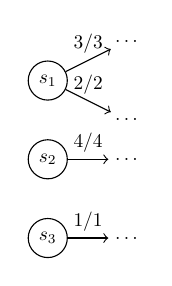
\begin{tikzpicture}[every node/.style={scale=.7}]
    \node [draw, circle] (s1) at (0, 2) {$s_1$};
    \node [draw, circle] (s2) at (0, 1) {$s_2$};
    \node [draw, circle] (s3) at (0, 0) {$s_3$};
    \node (v1) at (1, 2.5) {$\ldots$};
    \node (v2) at (1, 1.5) {$\ldots$};
    \node (v3) at (1, 1) {$\ldots$};
    \node (v4) at (1, 0) {$\ldots$};
    \draw [->] (s1) to node [above] {3/3} (v1);
    \draw [->] (s1) to node [above] {2/2} (v2);
    \draw [->] (s2) to node [above] {4/4} (v3);
    \draw [->] (s3) to node [above] {1/1} (v4);
  \end{tikzpicture}

  \end{tabular}
  \end{center}
\end{frame}

\begin{frame} \frametitle{Formulations for Robust Max-Flow}
From now on, we have the option of formulating problems as instances of the
more robust max-flow problem:
\stanza

\textbf{robust maximum flow problem} \\
\emph{input:} a flow network $G=(V,E),$ which may contain unreachable vertices,
antiparallel edges, a set $S \subseteq V$ of sources, and a set $T \subseteq V$
  of sinks\\
\emph{output:} a flow $f$ of maximum value $|f|$ \stanza

\end{frame}

\begin{frame} \frametitle{Bipartite Matching}
So far, all our reductions to max-flow have been either straightforward
flow simulations, or variations on max-flow. \stanza

Now we'll see a quite-different problem that also reduces to max-flow.
\end{frame}

\begin{frame} \frametitle{Partition of a Set}

  Intuitively: if $X = L \cup R$ is a \emph{partition,} then every element of $X$ is placed in $L$ or $R$ (but not both). \stanza

  Formally: $L$ and $R$ partition $X$ if
  \begin{itemize}
  \item $X = L \cup R,$
  \item $L \cap R = \emptyset,$ and
  \item $L \ne \emptyset, R \ne \emptyset.$
  \end{itemize}
  
\end{frame}

\begin{frame} \frametitle{Bipartite Matching}
\textbf{bipartite maximum matching} \\
\emph{input:} an undirected bipartite graph $G=(V, E)$ with parts $V=L \cup R$ \\
\emph{output:} a matching $M \subseteq E$ where the number of matched vertices
  is maximum \stanza

\begin{itemize}
  \item \emph{bipartite:} $L, R$ are disjoint and edges only go between $L, R$
  \item \emph{matching:} pick edges that ``pair off'' two vertices; goal is to
    maximize \#paired-off
  \item intuitively, $L$ is one kind of thing and $R$ is another kind of thing
\end{itemize}
\end{frame}

\begin{frame} \frametitle{Bipartite Matching}
\begin{center}
  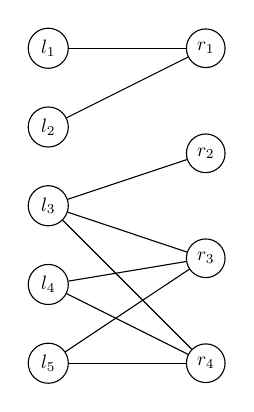
\begin{tikzpicture}[every node/.style={scale=.7}]

    \node [draw, circle] (l1) at (0, 4) {$l_1$};
    \node [draw, circle] (l2) at (0, 3) {$l_2$};
    \node [draw, circle] (l3) at (0, 2) {$l_3$};
    \node [draw, circle] (l4) at (0, 1) {$l_4$};
    \node [draw, circle] (l5) at (0, 0) {$l_5$};

    \node [draw, circle] (r1) at (2, 4) {$r_1$};
    \node [draw, circle] (r2) at (2, 2.666) {$r_2$};
    \node [draw, circle] (r3) at (2, 1.333) {$r_3$};
    \node [draw, circle] (r4) at (2, 0) {$r_4$};

    \draw (l1) to (r1);
    \draw (l2) to (r1);

    \draw (l3) to (r2);
    \draw (l3) to (r3);
    \draw (l3) to (r4);

    \draw (l4) to (r3);
    \draw (l4) to (r4);

    \draw (l5) to (r3);
    \draw (l5) to (r4);

  \end{tikzpicture}
\end{center}
\end{frame}

\begin{frame} \frametitle{Bipartite Matching}
\begin{center}
  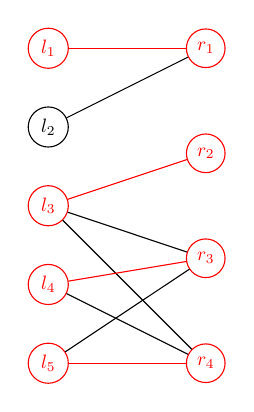
\begin{tikzpicture}[every node/.style={scale=.7}]

    \node [draw, circle, color=red] (l1) at (0, 4) {$l_1$};
    \node [draw, circle] (l2) at (0, 3) {$l_2$};
    \node [draw, circle, color=red] (l3) at (0, 2) {$l_3$};
    \node [draw, circle, color=red] (l4) at (0, 1) {$l_4$};
    \node [draw, circle, color=red] (l5) at (0, 0) {$l_5$};

    \node [draw, circle, color=red] (r1) at (2, 4) {$r_1$};
    \node [draw, circle, color=red] (r2) at (2, 2.666) {$r_2$};
    \node [draw, circle, color=red] (r3) at (2, 1.333) {$r_3$};
    \node [draw, circle, color=red] (r4) at (2, 0) {$r_4$};

    \draw [color=red] (l1) to (r1);
    \draw (l2) to (r1);

    \draw [color=red] (l3) to (r2);
    \draw (l3) to (r3);
    \draw (l3) to (r4);

    \draw [color=red] (l4) to (r3);
    \draw (l4) to (r4);

    \draw (l5) to (r3);
    \draw [color=red] (l5) to (r4);

  \end{tikzpicture}

  matching $M = \{\text{included edges}\}
    = \{ \{l_1, r_1\}, \{l_3, r_3\}, \{l_4, r_3\}, \{l_5, r_4\} \}$ \\

    $|M|=4$ \\

    (other optimal matchings exist)
\end{center}
\end{frame}

\begin{frame} \frametitle{Bipartite Matching Applications}
\begin{itemize}
  \item any scenario where there are two kinds of things that can be paired
  \item goal is simply maximum number of pairings
  \item casting for a play: $L = $ set of actors; $R = $ set of roles;
    edge $\{l, r\}$ exists when $l$ could play role $r$
  \item packing leftover food (one item/container): $L = $ set of food items; $R = $ available
    containers; edge $\{l, r\}$ exists when food $l$ could fit in container $r$
  \item scheduling appointments: $L = $ set of clients; $R = $ set of time slots;
    edge $\{l, r \}$ exists when client $l$ could meet appointment $r$
  \item might feel $NP$-hard, but actually in $P$
\end{itemize}
\end{frame}

\begin{frame} \frametitle{Formulating Bipartite Matching as Flow}
\begin{itemize}
  \item let $G=(V, E)$ be bipartite matching instance
  \item create $G'=(V', E')$ with $V' = V \cup \{s, t\}$ where $s, t$ are new
    source/sink
  \item create edges in $G'$:
  \begin{itemize}
    \item $(l, r) \enspace \forall l \in L, r \in R, \{l, r\} \in E$
    \item $(s, l) \enspace \forall l \in L$
    \item $(r, t) \enspace \forall r \in R$
  \end{itemize}
  \item every edge $(v, w)$ has capacity $c(v, w)=1$
  \item post-processing: edge $(l, r) \in M$ iff $f(l, r)=1$
  \item observe $|V'| \in O(|V|), |E'| \in O(|E|),$ overhead is $O(|V|+|E|)$
  \item $\implies$ if this is correct, can solve bipartite matching in $O(|V|^3)$ time
\end{itemize}
\end{frame}

\begin{frame} \frametitle{Formulating Bipartite Matching as Flow}
  \begin{center}
  \begin{tabular}{cccc}
  $G$ & $G'$ & $f'$ & $M$ \\

  % G
  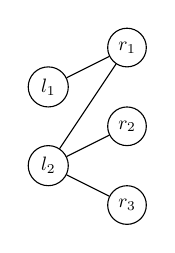
\begin{tikzpicture}[every node/.style={scale=.7}]
    \node [draw, circle] (l1) at (0, 1.5) {$l_1$};
    \node [draw, circle] (l2) at (0, .5) {$l_2$};
    \node [draw, circle] (r1) at (1, 2) {$r_1$};
    \node [draw, circle] (r2) at (1, 1) {$r_2$};
    \node [draw, circle] (r3) at (1, 0) {$r_3$};
    \draw (l1) to (r1);
    \draw (l2) to (r1);
    \draw (l2) to (r2);
    \draw (l2) to (r3);
  \end{tikzpicture}

  % G'
  &
  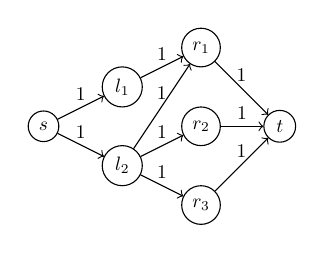
\begin{tikzpicture}[every node/.style={scale=.7}]
    \node [draw, circle] (l1) at (0, 1.5) {$l_1$};
    \node [draw, circle] (l2) at (0, .5) {$l_2$};
    \node [draw, circle] (r1) at (1, 2) {$r_1$};
    \node [draw, circle] (r2) at (1, 1) {$r_2$};
    \node [draw, circle] (r3) at (1, 0) {$r_3$};

    \node [draw, circle] (s) at (-1, 1) {$s$};
    \node [draw, circle] (t) at (2, 1) {$t$};

    \draw [->] (l1) to node [above] {1} (r1);
    \draw [->] (l2) to node [above] {1} (r1);
    \draw [->] (l2) to node [above] {1} (r2);
    \draw [->] (l2) to node [above] {1} (r3);

    \draw [->] (s) to node [above] {1} (l1);
    \draw [->] (s) to node [above] {1} (l2);
    \draw [->] (r1) to node [above] {1} (t);
    \draw [->] (r2) to node [above] {1} (t);
    \draw [->] (r3) to node [above] {1} (t);
  \end{tikzpicture}

  % f'
  &
  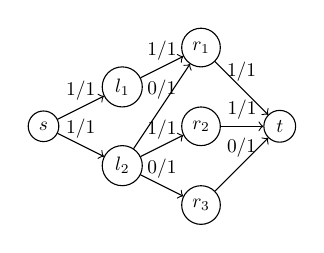
\begin{tikzpicture}[every node/.style={scale=.7}]
    \node [draw, circle] (l1) at (0, 1.5) {$l_1$};
    \node [draw, circle] (l2) at (0, .5) {$l_2$};
    \node [draw, circle] (r1) at (1, 2) {$r_1$};
    \node [draw, circle] (r2) at (1, 1) {$r_2$};
    \node [draw, circle] (r3) at (1, 0) {$r_3$};

    \node [draw, circle] (s) at (-1, 1) {$s$};
    \node [draw, circle] (t) at (2, 1) {$t$};

    \draw [->] (l1) to node [above] {1/1} (r1);
    \draw [->] (l2) to node [above] {0/1} (r1);
    \draw [->] (l2) to node [above] {1/1} (r2);
    \draw [->] (l2) to node [above] {0/1} (r3);

    \draw [->] (s) to node [above] {1/1} (l1);
    \draw [->] (s) to node [above] {1/1} (l2);
    \draw [->] (r1) to node [above] {1/1} (t);
    \draw [->] (r2) to node [above] {1/1} (t);
    \draw [->] (r3) to node [above] {0/1} (t);
  \end{tikzpicture}

    % M
    &
    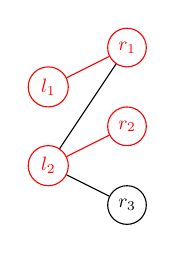
\begin{tikzpicture}[every node/.style={scale=.7}]
      \node [draw, circle, color=red] (l1) at (0, 1.5) {$l_1$};
      \node [draw, circle, color=red] (l2) at (0, .5) {$l_2$};
      \node [draw, circle, color=red] (r1) at (1, 2) {$r_1$};
      \node [draw, circle, color=red] (r2) at (1, 1) {$r_2$};
      \node [draw, circle] (r3) at (1, 0) {$r_3$};
      \draw [color=red] (l1) to (r1);
      \draw (l2) to (r1);
      \draw [color=red] (l2) to (r2);
      \draw (l2) to (r3);
    \end{tikzpicture}

  \end{tabular}
  \vspace{.5cm}
  $M = \{ \{l, r\} \, | \, f'(l, r)=1 \} = \{ \{l_1, r_1\}, \{l_2, r_2\} \}$ \\
  (other max flows $\Leftrightarrow$ matchings exist)
  \end{center}
\end{frame}

\begin{frame} \frametitle{Correctness of this Formulation}
Technical details:
\begin{itemize}
  \item \emph{integrality theorem:} if every capacity $c(u, v) \in \mathbb{Z}$
    then every $f(u, v) \in \mathbb{Z}$ and $|f| \in \mathbb{Z}$
  \item $\exists$ matching $M$ with cardinality $k=|M|$ iff $\exists$ some flow $f$
    with value $k=|f|$
    \begin{itemize}
      \item key idea: pairing two vertices in the matching adds exactly one
        flow from $s \leadsto t$
      \item there are no opportunities for flow aside from matched vertices
    \end{itemize}
  \item $\implies$ a maximum flow in $G'$ corresponds to a maximum matching in $G$
\end{itemize}
\end{frame}

\begin{frame} \frametitle{Summary}
  \begin{itemize}
    \item classical max-flow problem can be solved in $O(|V|^3)$ time, in $P$
    \item robust max-flow problem (supports unreachable vertices, antiparallel edges, multiple sinks/sources)
      also in $O(|V|^3)$ time w/ worse constant factors, in $P$
    \item bipartite matching reduces to max-flow, so bipartite matching can be solved in
      $O(|V|^3)$ time, in $P$
    \item other practical, distinct problems reduce to max-flow or bipartite
      matching so take $O(|V|^3)$ time and are in $P$
  \end{itemize}
\end{frame}

\end{document}
